\section{Why are tensors so sigma!}
Nakahara defines tensor as:
\begin{quote}
    \textit{A tensor $T$ of type $(p,q)$ is a multi-linear map that maps $q$ vectors and $p$ dual vectors to $\mathbb{R}$, that is:
    $$ T: \brac{\bigotimes\limits^p \mathbf{V}^* }\bigotimes \brac{\bigotimes\limits^q \mathbf{V} }\to \mathbb{R} $$}
\end{quote}
Dayummm!! \emoji{expressionless-face} Let us break this down. Consider a scalar which has no vector and no dual vector. Thus, it is a $(0,0)$ type tensor. Now, let us consider a vector $\mathbf{v}$. This is a $(1,0)$ tensor, that is, it maps a dual vector to a scalar. If we have a dual vector $\mathbf{f}$, then it is of type $(0,1)$ and maps a vector to a scalar. This does not clear anything. Let us instead consider few examples:\\[0.3cm]
\textbf{Moment of Intertia Tensor:}\\[0.3cm]
Perhaps the first example of a tensor we had encountered during our classical mechanics course (which we had been told to understand just as a `matrix'). 
\begin{figure}[H]
    \centering
    

\tikzset{every picture/.style={line width=0.75pt}} %set default line width to 0.75pt        

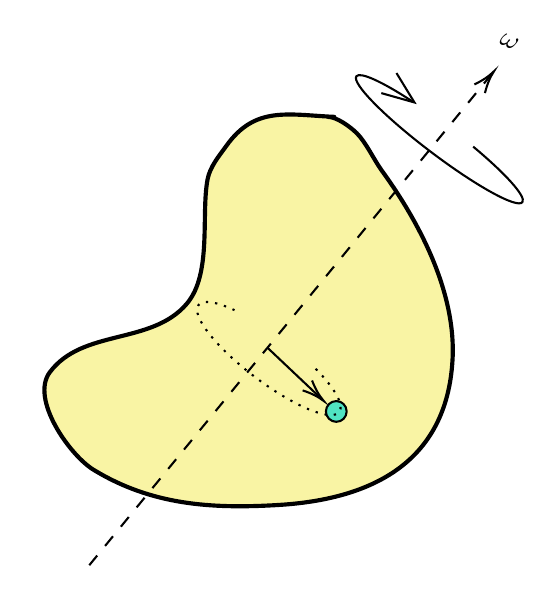
\begin{tikzpicture}[x=0.75pt,y=0.75pt,yscale=-1,xscale=1]
%uncomment if require: \path (0,300); %set diagram left start at 0, and has height of 300

%Curve Lines [id:da6245196964627165] 
\draw [fill={rgb, 255:red, 245; green, 236; blue, 95 }  ,fill opacity=0.57 ][line width=1.5] [line join = round][line cap = round]   (279,53.63) .. controls (256.55,52.61) and (240.86,48.23) .. (227,67.63) .. controls (223.44,72.61) and (219.16,77.63) .. (218,83.63) .. controls (214.73,100.51) and (220.24,129.16) .. (208,143.63) .. controls (191.03,163.69) and (157.82,155.54) .. (142,176.63) .. controls (132.31,189.55) and (151.65,216.7) .. (163,223.63) .. controls (190.78,240.61) and (219.54,242.57) .. (252,240.63) .. controls (296.26,237.99) and (333.22,220.66) .. (336,170.63) .. controls (337.8,138.31) and (320.09,104.5) .. (302,79.63) .. controls (298.32,74.58) and (294.26,65.9) .. (290,61.63) .. controls (286.43,58.06) and (280,53.65) .. (276,53.63) ;
%Straight Lines [id:da1466264621432246] 
\draw  [dash pattern={on 4.5pt off 4.5pt}]  (161,269.63) -- (354.73,33.18) ;
\draw [shift={(356,31.63)}, rotate = 129.33] [color={rgb, 255:red, 0; green, 0; blue, 0 }  ][line width=0.75]    (10.93,-3.29) .. controls (6.95,-1.4) and (3.31,-0.3) .. (0,0) .. controls (3.31,0.3) and (6.95,1.4) .. (10.93,3.29)   ;
%Shape: Arc [id:dp5966527947933914] 
\draw  [draw opacity=0] (345.95,67.97) .. controls (361.58,81) and (371.64,92.13) .. (369.66,94.74) .. controls (367.21,97.97) and (347.32,87) .. (325.24,70.25) .. controls (303.15,53.49) and (287.24,37.29) .. (289.69,34.06) .. controls (291.47,31.72) and (302.46,36.86) .. (316.8,46.28) -- (329.67,64.4) -- cycle ; \draw   (345.95,67.97) .. controls (361.58,81) and (371.64,92.13) .. (369.66,94.74) .. controls (367.21,97.97) and (347.32,87) .. (325.24,70.25) .. controls (303.15,53.49) and (287.24,37.29) .. (289.69,34.06) .. controls (291.47,31.72) and (302.46,36.86) .. (316.8,46.28) ;  
\draw   (309,32.52) -- (317.66,46.69) -- (301.68,42.18) ;
%Straight Lines [id:da4118334667699356] 
\draw    (247,165) -- (272.55,189.18) ;
\draw [shift={(274,190.55)}, rotate = 223.42] [color={rgb, 255:red, 0; green, 0; blue, 0 }  ][line width=0.75]    (10.93,-3.29) .. controls (6.95,-1.4) and (3.31,-0.3) .. (0,0) .. controls (3.31,0.3) and (6.95,1.4) .. (10.93,3.29)   ;
%Shape: Circle [id:dp5534282668246396] 
\draw  [fill={rgb, 255:red, 80; green, 227; blue, 194 }  ,fill opacity=1 ] (275,195.55) .. controls (275,192.79) and (277.24,190.55) .. (280,190.55) .. controls (282.76,190.55) and (285,192.79) .. (285,195.55) .. controls (285,198.31) and (282.76,200.55) .. (280,200.55) .. controls (277.24,200.55) and (275,198.31) .. (275,195.55) -- cycle ;
%Shape: Arc [id:dp400640896970585] 
\draw  [draw opacity=0][dash pattern={on 0.84pt off 2.51pt}] (270.08,175) .. controls (279.21,184.33) and (283.96,192.49) .. (281.44,195.8) .. controls (277.72,200.7) and (259.52,193.15) .. (240.78,178.93) .. controls (222.04,164.72) and (209.86,149.22) .. (213.58,144.31) .. controls (215.66,141.57) and (222.27,142.72) .. (230.96,146.75) -- (247.51,170.06) -- cycle ; \draw  [dash pattern={on 0.84pt off 2.51pt}] (270.08,175) .. controls (279.21,184.33) and (283.96,192.49) .. (281.44,195.8) .. controls (277.72,200.7) and (259.52,193.15) .. (240.78,178.93) .. controls (222.04,164.72) and (209.86,149.22) .. (213.58,144.31) .. controls (215.66,141.57) and (222.27,142.72) .. (230.96,146.75) ;  

% Text Node
\draw (359.85,11.16) node [anchor=north west][inner sep=0.75pt]  [rotate=-24.91]  {$\omega $};


\end{tikzpicture}

    \caption{A rigid body rotating about an axis}
\end{figure}
\noindent
Consider a rigid body made of tiny masses $dm$. Consider one such mass sitauted as a distance $s$ from the fixed axis of rotation. It goes around a circle with speed $v = \omega s$. The angular momentum can be calculated as:
$$\mathbf{L} = \int (\veb{r}\times \veb{v})dm = \int (\veb{r}\times (\veb{\omega}\times \veb{r}))dm = \int (\veb{r}\cdot \veb{r})\veb{\omega} -  \cancelto{0}{(\veb{r}\cdot \veb{\omega})}\veb{r}dm =\veb{\omega} \underbrace{\int s^2 dm}_{\text{I}} $$
The integral is called the moment of inertia. In a more general case, where there is no fixed axis of rotation, we write: 
\begin{align*}
    \mathbf{L} &= \int (\veb{r}\times \veb{v})dm \\
    &= \int (\veb{r}\times (\veb{\omega}\times \veb{r}))dm \\
    &= \int (\veb{r}\cdot \veb{r})\veb{\omega} -  {(\veb{r}\cdot \veb{\omega})}\veb{r}dm
\end{align*}
We now write it in index notation, noting that $\omega^i = \tensor*{\delta}{^i^j}\omega_j$:
\begin{align*}
    L^i &= \int (\veb{r}\cdot \veb{r})\tensor*{\delta}{^i^j}\omega_j - x^i(x^j\omega_j)dm\\
    &= \omega_j \brac{\int (\veb{r}\cdot \veb{r})\tensor*{\delta}{^i^j} - x^ix^j\ dm} 
\end{align*}
The integral in the bracket is defined to be the inertia tensor:
$$I^{ij} = \int (\veb{r}\cdot \veb{r})\tensor*{\delta}{^i^j} - x^ix^j \ dm$$
Note that $i$ and $j$ goes from $1$ to $3$ and thus it has $9$ components but since the expression is symmetric, we only have $6$ independent components. This states that the angular momentum and the angular velocity are not necessarily parallel in some coordinate system where $I$ have non-zero off-diagonal entries.\\[0.3cm]
\textbf{Electromagnetic Tensor:}\\[0.3cm]
The electromagnetic tensor is very useful in combining the electric field and magnetic field and finding their transformations. It is defined as:
$$F_{\mu\nu} = \partial_\mu A_\nu - \partial_\nu A_\mu$$
where $A_\mu$ is the 4-potential. The indices $\mu$ and $\nu$ can take values from $0$ to $3$. The tensor has $16$ components but only $6$ of them are independent. The tensor is antisymmetric, that is, $F_{\mu\nu} = -F_{\nu\mu}$ and thus the diagonal entries are zero. We will discuss this later but Maxwell's equations can be written in a very compact form using the components of the electromagnetic tensor.\\[0.3cm]
\textbf{Electric-Susceptibility Tensor:}\\[0.3cm]
We had studied about polarisation in dielectrics in our classical electrodynamics course where we had often taken (for simplicity):
$$\veb{P} = \epsilon_0\chi\veb{E}$$
Here we had taken the electric field to be parallel to the polarisation vector but in general, these are related by the susceptibility tensor as:
$$P^i = \epsilon_0\chi^{ij}E^{j}$$
\subsection{Gradient}
The components of the gradient (basically partial derivative) are covariant. We denote it with a lower index explicitly to show that it is a covariant vector:
$$\partial_\mu \equiv \pdv{x^\mu}$$
Then accordingly we will have:
$$\partial^\mu \equiv \pdv{x_\mu} \quad \quad \partial^\mu = g^{\mu\nu}\partial_\nu$$
\subsection{Tensor Transformations}
As previously seen for vector transformation, the transformation of a tensor from one system to another is very similar. For simplicity, we show for a second rank tensor:
$$\tensor{T }{^{\prime ij}} = \pdv{x^{\prime i}}{x^k} \pdv{x^{\prime j}}{x^n} \tensor{T}{^{kn}}$$
This is simple: in the left everything is prime and contravariant, so in the right the numerator must have primes and the denominator must have unprimed indices and contraction should be done so as to match the contra and co indices on both sides in the final expansion. Well, this transformation law is such a nice thing that many people say that: 
$$\boxed{\mathrm{Tensors\ are \ defined\ in\ the\ way\ they\ transform}}$$
Let us see some more examples of tensors and their transformation from lower to upper indices (it's easy, just use the metric tensor appropriately):
\begin{align*}
    \tensor{T}{^\mu^\nu} &=g^{\rho\mu}g^{\sigma\nu} \tensor{T}{_\rho_\sigma}\\
    \tensor{T}{^\mu _\nu} &=\tensor{g}{^\mu _\rho}\tensor{g}{^\sigma _\nu} \tensor{T}{^\rho _\sigma}
\end{align*}
Lastly we show an example of a mixed tensor transformation from one system to another \emoji{fire}:
\begin{align*}
    \tensor{T}{^{\prime\mu} _\nu _\rho} =\pdv{x^\beta}{x'^\rho}\ \pdv{x^\alpha}{x'^\nu} \ \pdv{x'^\mu}{x^\sigma}  \tensor{T}{^\sigma _\alpha _\beta}
\end{align*}
So basically, while changing the covariant indices, the prime is in the denominator and for contravariant, it is above. And then the positioning of the indices is trivial (I guess...)
\subsection{Matrices vs. Tensor? same same but different....}
Not all matrices are second-rank tensors \emoji{expressionless}. Yes, the components of a second-rank tensor can be arranged in a matrix form but there are many matrices which do not transform according to the above equation. Take for example the following matrix, which we assume as a tensor:
$$[T^{lm}] \equiv \begin{pmatrix}
    (x^2)^2 & x^1x^2\\
    x^1x^2 & (x^2)^2
\end{pmatrix}$$
Note that the 2 outside the bracket is the power and inside the bracket is the index of the component. Then after rotation, we have the following relation:
\begin{align*}
    x'^1 &= x^1\cos\theta + x^2\sin\theta \\
    x'^2 &= -x^1\sin\theta + x^2\cos\theta
\end{align*}
Let us find $T^{'11}$ which according to the transformation rule, should be:
\begin{align*}
    T^{'11} &= \pdv{x'^1}{x^k} \pdv{x'^1}{x^n} T^{kn} \\
    &=\pdv{x'^1}{x^1} \pdv{x'^1}{x^1} T^{11} + \pdv{x'^1}{x^1} \pdv{x'^1}{x^2} T^{12}+\pdv{x'^1}{x^2} \pdv{x'^1}{x^1} T^{21} +\pdv{x'^1}{x^2} \pdv{x'^1}{x^2}T^{22}\\
    &= \cos\theta\cos\theta T^{11} + \cos\theta \sin\theta T^{12} + \sin\theta\cos\theta T^{21} + \sin\theta\sin\theta T^{22} \\
    &= \cos^2\theta (x^2)^2 + 2\sin\theta\cos\theta (x^1)(x^2) + \sin^2\theta (x^2)^2\\
    &=(x^2\cos\theta + x^1\sin\theta)^2
\end{align*}
Well note that if $T$ was indeed a tensor, then $T^{'11}$ should be equal to $(x'^2)^2$ but it is not. Thus, $T$ is not a tensor and our assumption was wrong.  \textbf{Thus all matrices are not tensors!}